\subsection{Top Agents and Trends} \label{viztopagents}
Website traffic is mainly attributed to the  various requests that are made to the server hosting the content. Let us review the requests made for scimaps.org. 
We have data of top 15 user agents from March-2007 to Jan-2017.  
Judging by the yearly pattern of the number of hits, we can mark 2011 as the pinnacle, after successive unremarkable hit fluctuations from 2007-10. there was a record 115$\%$ increase in the hits as compared to 2010. And the year 2012 was even better with a ~21$\%$ increase over 2011. But since then the website has observed a downfall. The year 2013-14-15 have all marked the negative trend in the number of visitors/requests made for the site. Justifying a need for a website overhaul in 2015. We observe an increase of ~10$\%$ in the request in the subsequent year. And the positive trend seems to be continuing as January records an increase of ~26$\%$  over Dec-2016.
Let us dive deeper and inspect the terminals that are making these requests. We have observed 6 types of terminals that attribute to the traffic on scimaps.org, the are:
\begin{itemize}
\item Windows PC
\item Macintosh
\item Linux Terminals
\item iPhone
\item iPad
\item Bots
\end{itemize}

\begin{figure}
\centering
\fbox{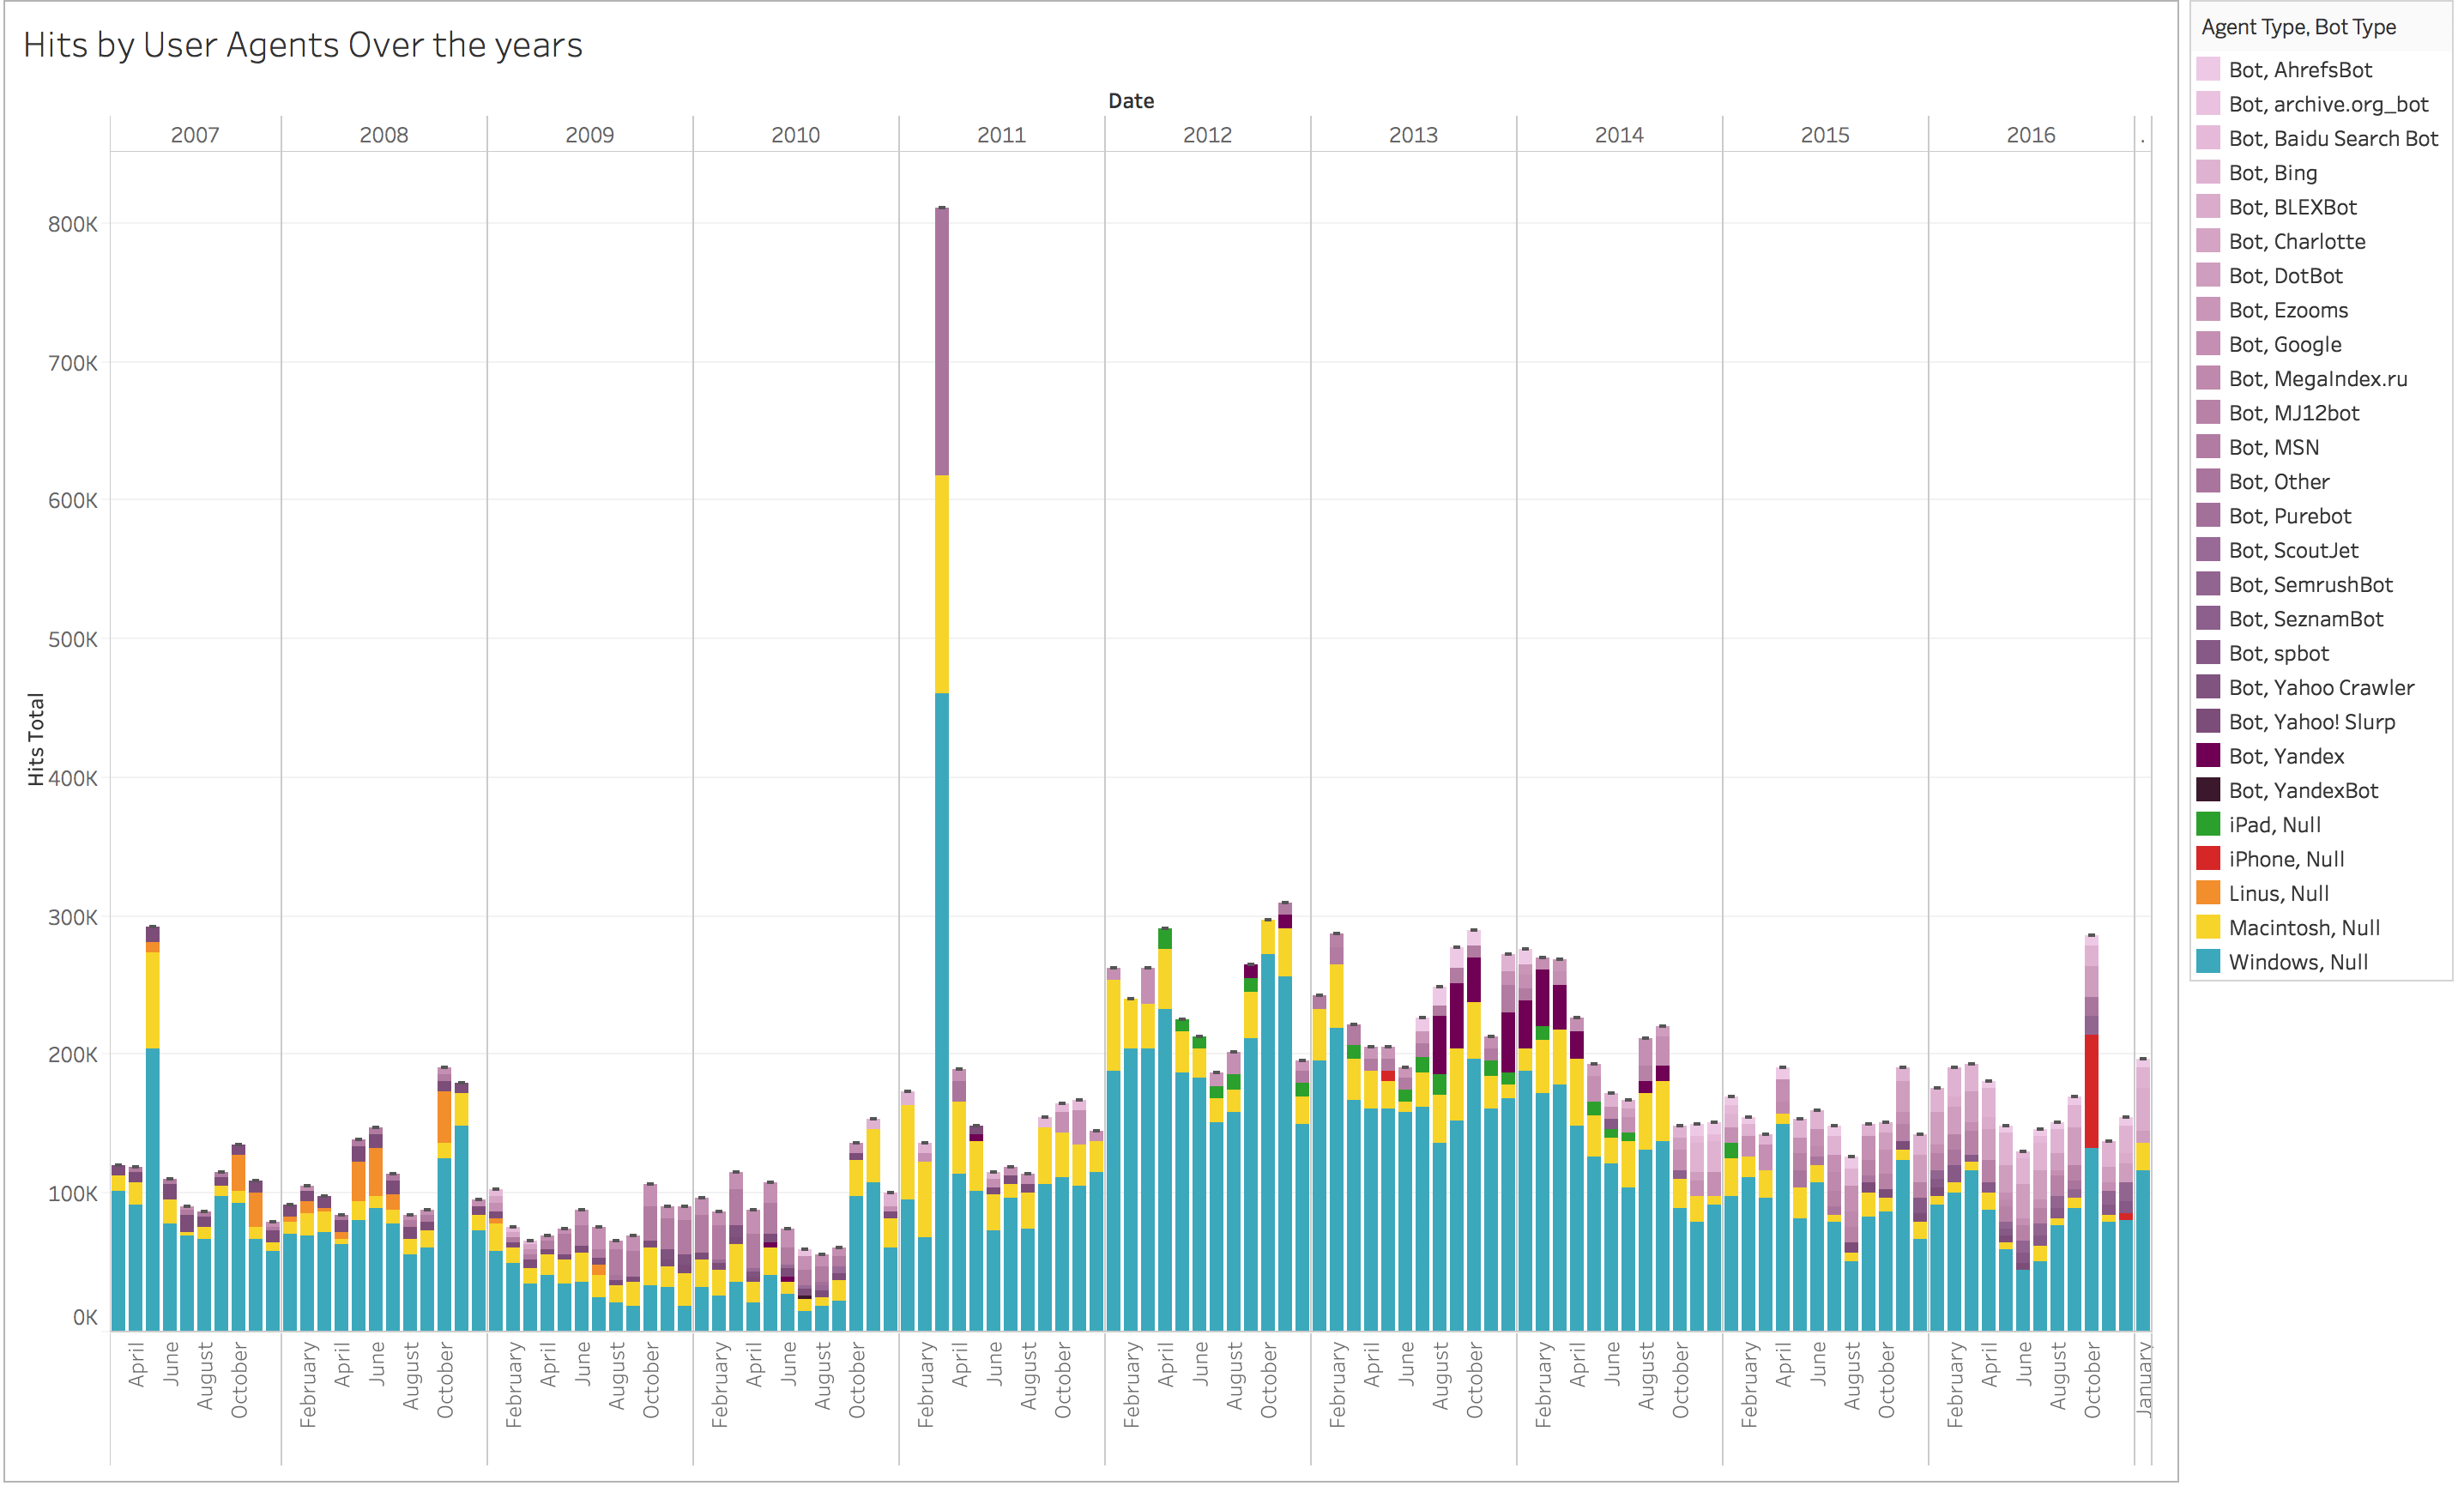
\includegraphics[width=\linewidth]{img/TopAgents.png}}
\caption{Accessing scimaps.org Traffic (2007 - 2017)}
\label{fig:TopAgents}
\end{figure}

We see that the majority of traffic seems to be coming from Windows PC during the majority of 2007 - 2015. But, the hits/requests made by other terminals/bots seems to be catching up and the share evens out after the website’s overhaul. Till 2015 we observe that majority of traffic is from windows users, the traffic made by bots appears to have risen during this time. After the overhaul, Windows and bots share an approximate equal share of the website traffic, with mac traffic share increasing to 10.32$\%$ in 2017 over 2016. 
Of all the bots, major traffic should be attributed to Google, Yahoo Slurp and MSN bots from 2007 - 2010. And, in recent past DotBot and Bing seems to be the prime bots making 11.59$\%$ and ~11$\%$ of traffic in 2016 respectively.
